\label{ch:simulations}

The previous chapter explained that the history of the neutron noise method began as part of the core diagnostics methods performed in a nuclear reactor. Seeing the success of the technique, computational methods to solve the neutron noise have also been developed \cite{demaziereCORTEXProjectImproving2020}. To perform reactor diagnostics using neutron noise analysis computationally, the tool must have the capability to perform neutron noise calculations, forward flux calculations, and generate the Green’s function matrix. The forward flux is part of the source term in the neutron noise equation, which will be shown in the next section. The Green’s function is used as part of the neutron noise unfolding method. The adjoint flux is used to determine the characteristics of neutron noise (e.g. neutron noise components and ZPRTF) as shown in Section \ref{sec:noise_derivation}. Numerous efforts have been made to computationally solve the neutron noise equation. Several examples of tools have been mentioned in the previous chapter.

Forward, adjoint, neutron noise, and Green's function simulator is not a unique problem to solve. There has been many tool developed for these purposes. Tools such as CORE SIM+ \cite{mylonakisCORESIMFlexible2021} can perform forward, adjoint, and noise calculations, as well as generate the Green’s function matrix. Another tool, such as FEMFFUSION \cite{vidal-ferrandizFEMFFUSIONFiniteElement2023}, can perform forward, adjoint, and noise calculations for rectangular and triangular mesh using a finite element method. Other examples of tools have been mentioned in Section \ref{sec:noise_tools}. In this dissertation, a numerical tool for neutron noise analysis is developed to ensure a consistency between the solutions of forward flux, adjoint flux, neutron noise, and the Green's function. By developing a unified numerical tool, all four calculations share the same numerical framework, discretization, and data structures, eliminating discrepancies that can arise when mixing external tools with different discretization strategies. The tool is based on on a multigroup diffusion equation and a finite volume method for spatial discretization. The tool is available in \href{https://github.com/harunardi/FANGS-UNFOLD}{GitHub}\footnote{https://github.com/harunardi/FANGS-UNFOLD} for future references.

The structure of this chapter is as follows. First, we review the neutron noise equation, which was derived in the previous chapter. This includes the forward and adjoint equations, as well as the inputs and outputs for each equation. Then, we focus on the spatial discretization method using the finite volume method and how it is applied to 3D triangular geometries for each equation. We also explain the boundary conditions that can be used in the tool. Lastly, we provide some case examples for verifying the tool.

\section{The Neutron Noise Equation}
The neutron noise equation has been derived in the previous chapter. The equation is given in Eq. \ref{eq:freq_4}, which is repeated here for convenience:
\begin{equation}
        \begin{aligned}
                \frac{i \omega}{v_g} \delta \phi_g (\textbf{r}, \omega) - \nabla D_g(\textbf{r}) \nabla \delta \phi_g(\textbf{r}, \omega) + \Sigma_{t,g,0}(\textbf{r}) \delta \phi_g(\textbf{r}, \omega) - \sum_{g' = 1}^{G} \biggl(\Sigma_{s0,g',g,0}(\textbf{r}) \delta \phi_{g'}(\textbf{r}, \omega) \biggr) -\\ \frac{1}{k_{\text{eff}}} \biggl( \chi^p_g (1-\beta_{\text{eff}}) + \chi^d_g \frac{\lambda \beta_{\text{eff}}}{i \omega + \lambda} \biggr)  \biggl(\sum_{g' = 1}^{G} \nu \Sigma_{f,g',0}(\textbf{r}) \delta \phi_{g'}(\textbf{r}, \omega) \biggr)= \\
                - \delta \Sigma_{t,g}(\textbf{r}, \omega) \phi_{g,0}(\textbf{r}) + \sum_{g' = 1}^{G} \biggl(\delta \Sigma_{s0,g',g}(\textbf{r}, \omega) \phi_{g',0}(\textbf{r}) \biggr)\\
                \frac{1}{k_{\text{eff}}} \biggl( \chi^p_g (1-\beta_{\text{eff}}) + \chi^d_g \frac{\lambda \beta_{\text{eff}}}{i \omega + \lambda} \biggr)  \biggl( \sum_{g' = 1}^{G} \delta \nu \Sigma_{f,g'}(\textbf{r}, \omega) \phi_{g',0}(\textbf{r}) \biggr)
        \end{aligned}
        \label{eq:freq_4_ch3}
\end{equation}
Eq. \ref{eq:freq_4_ch3} shows the multigroup neutron noise equation in the frequency domain, where $\delta \phi_g (\textbf{r}, \omega)$ is the group-wise neutron noise and $\omega$ is the angular frequency (radians per second). The unknown (output) of the equation is the neutron noise, $\delta \phi_g (\textbf{r}, \omega)$ with unit of $\frac{n}{cm^2}$, the knowns (inputs) are the macroscopic cross sections and the noise source.

In Eq. \ref{eq:freq_4_ch3}, the noise source is defined as the combination of perturbed macroscopic cross sections and the forward flux $\phi_{g,0} (\textbf{r})$. The forward flux is obtained from the steady-state multigroup neutron diffusion equation \cite{duderstadtNuclearReactorAnalysis1977}, shown in Eq. \ref{eq:forward_eq_ch3}.
\begin{equation}
        \begin{aligned}
                - \nabla D_g(\textbf{r}) \nabla \phi_{g,0}(\textbf{r}) + \Sigma_{t,g,0}(\textbf{r}) \phi_{g,0}(\textbf{r}) = \sum_{g' = 1}^{G} \biggl(\Sigma_{s0,g',g,0}(\textbf{r}) \phi_{g',0}(\textbf{r}) \biggr) \\
                + \frac{1}{k_{\text{eff}}} \biggl( \chi^p_g (1-\beta_{\text{eff}}) + \chi^d_g \beta_{\text{eff}} \biggr)  \biggl( \sum_{g' = 1}^{G} \nu \Sigma_{f,g',0}(\textbf{r}) \phi_{g',0}(\textbf{r}) \biggr)
        \end{aligned}
        \label{eq:forward_eq_ch3}
\end{equation}
In Eq. \ref{eq:forward_eq_ch3}, the knowns (input) are the macroscopic cross sections, the unknown (outputs) are the forward flux and the criticality $k_{\text{eff}}$. 

The tool also solve the multigroup adjoint equation \cite{duderstadtNuclearReactorAnalysis1977}, as it is important for calculating the neutron noise components and zero-power reactor transfer function:
\begin{equation}
        \begin{aligned}
                - \nabla D_g(\textbf{r}) \nabla \phi^{\dagger}_{g,0}(\textbf{r}) + \Sigma_{t,g,0}(\textbf{r}) \phi^{\dagger}_{g,0}(\textbf{r}) = \sum_{g' = 1}^{G} \biggl(\Sigma_{s0,g,g',0}(\textbf{r}) \phi^{\dagger}_{g',0}(\textbf{r}) \biggr) \\
                + \frac{1}{k_{\text{eff}}} \nu \Sigma_{f,g,0}(\textbf{r}) \biggl( \sum_{g' = 1}^{G} \bigl( \chi^p_{g'} (1-\beta_{\text{eff}}) + \chi^d_{g'} \beta_{\text{eff}} \bigr) \phi^{\dagger}_{g',0}(\textbf{r}) \biggr)
        \end{aligned}
        \label{eq:adjoint_eq_ch3}
\end{equation}
Here, the known (inputs) are the macroscopic cross sections, the unknown (outputs) are the adjoint flux and the criticality $k_{\text{eff}}$.

\section{The Neutron Noise tool}

\subsection{Spatial Discretization for Triangular Geometries}

In this chapter, the 3D system for triangular geometries are derived. The neutron noise tool is developed using the finite volume method as the spatial discretization method. In case of hexagonal assembly, it is divided into 6 equilateral triangles, and mesh refinement is done by subdividing each triangle into 4 equilateral triangles. The total number of triangles in the hexagon is defined as follows:
\begin{equation}
    n = 6 \times 4^{\text{level}}
\end{equation}
where “level” is the mesh refinement level, which indicates how many times the triangular meshes have been subdivided. This means that level 0 consists of 6 triangles (no subdivision), level 1 consists of 24 triangles (subdivided once), level 2 consists of 96 triangles (subdivided twice), and so on. Figure \ref{fig:2DTri discretization} shows how the indexing of the triangular grid works. The visual representation of the discretization for 3D triangular geometries is shown in Figure \ref{fig:3DTri discretization}.

\begin{figure}[H]
        \centering
        \begin{subfigure}{.48\textwidth}
          \centering
          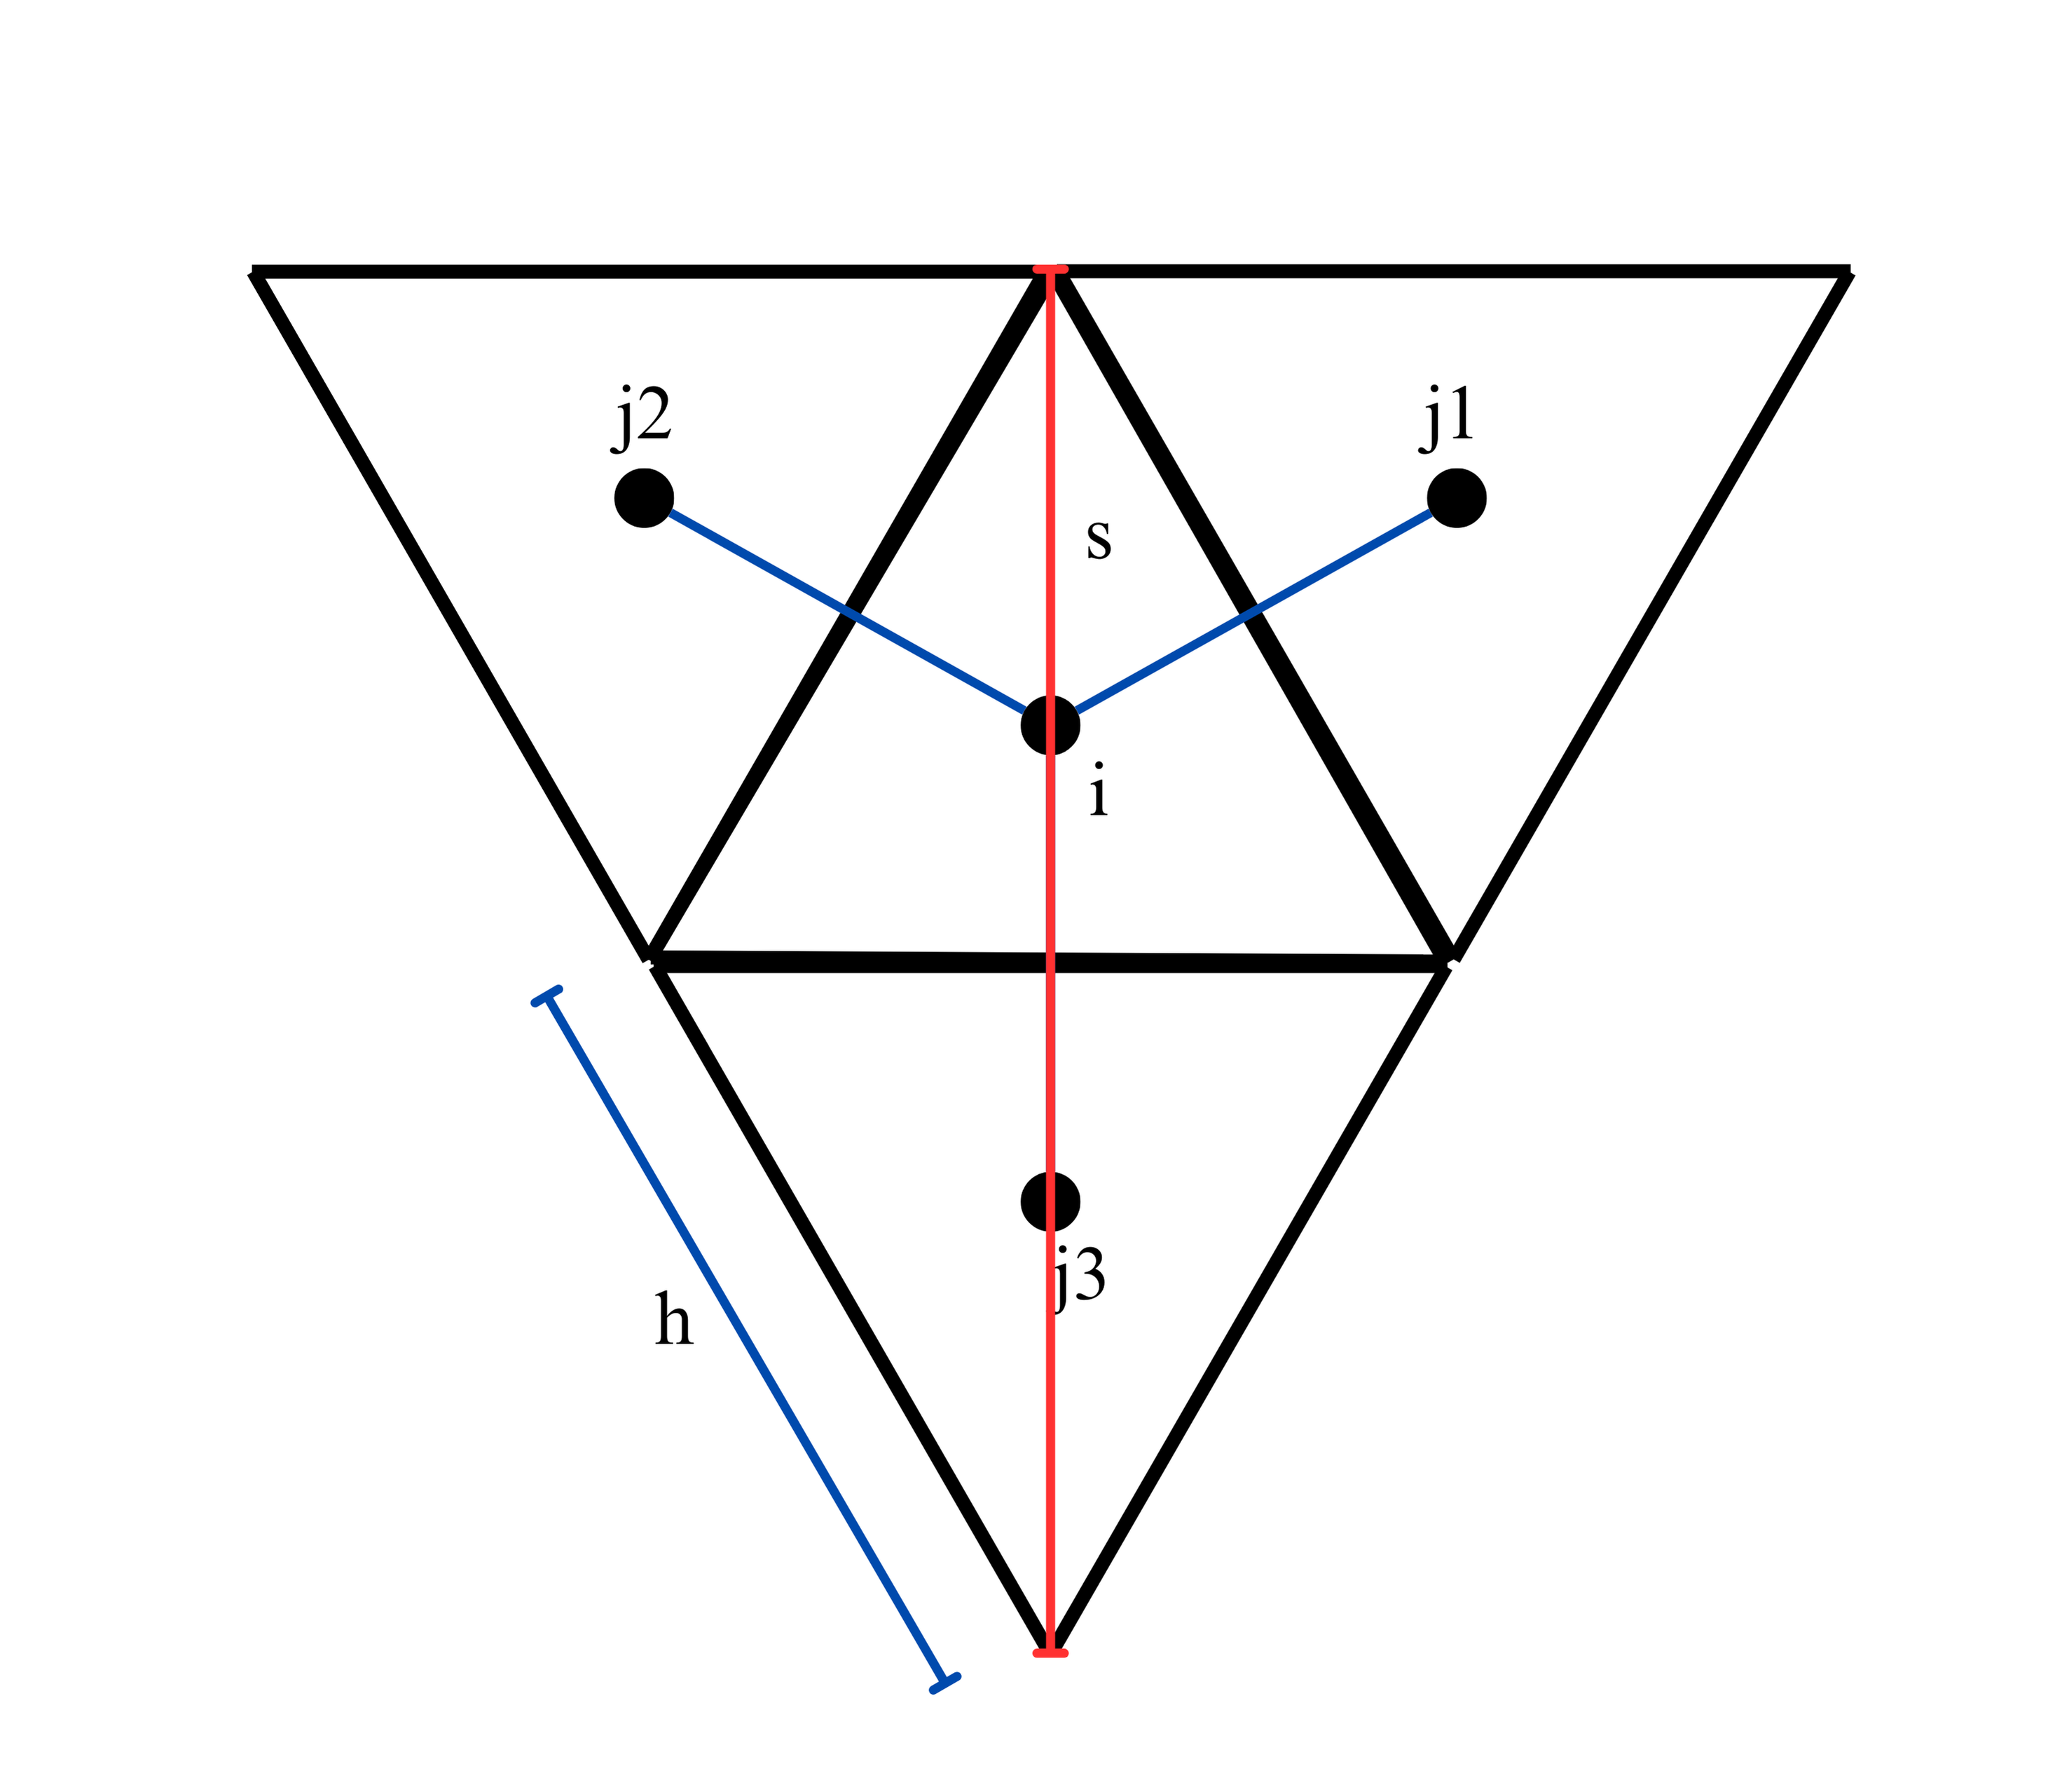
\includegraphics[width=\linewidth]{figures/disc_hexx.png}
        \end{subfigure}
        \hfill
        \begin{subfigure}{.48\textwidth}
          \centering
          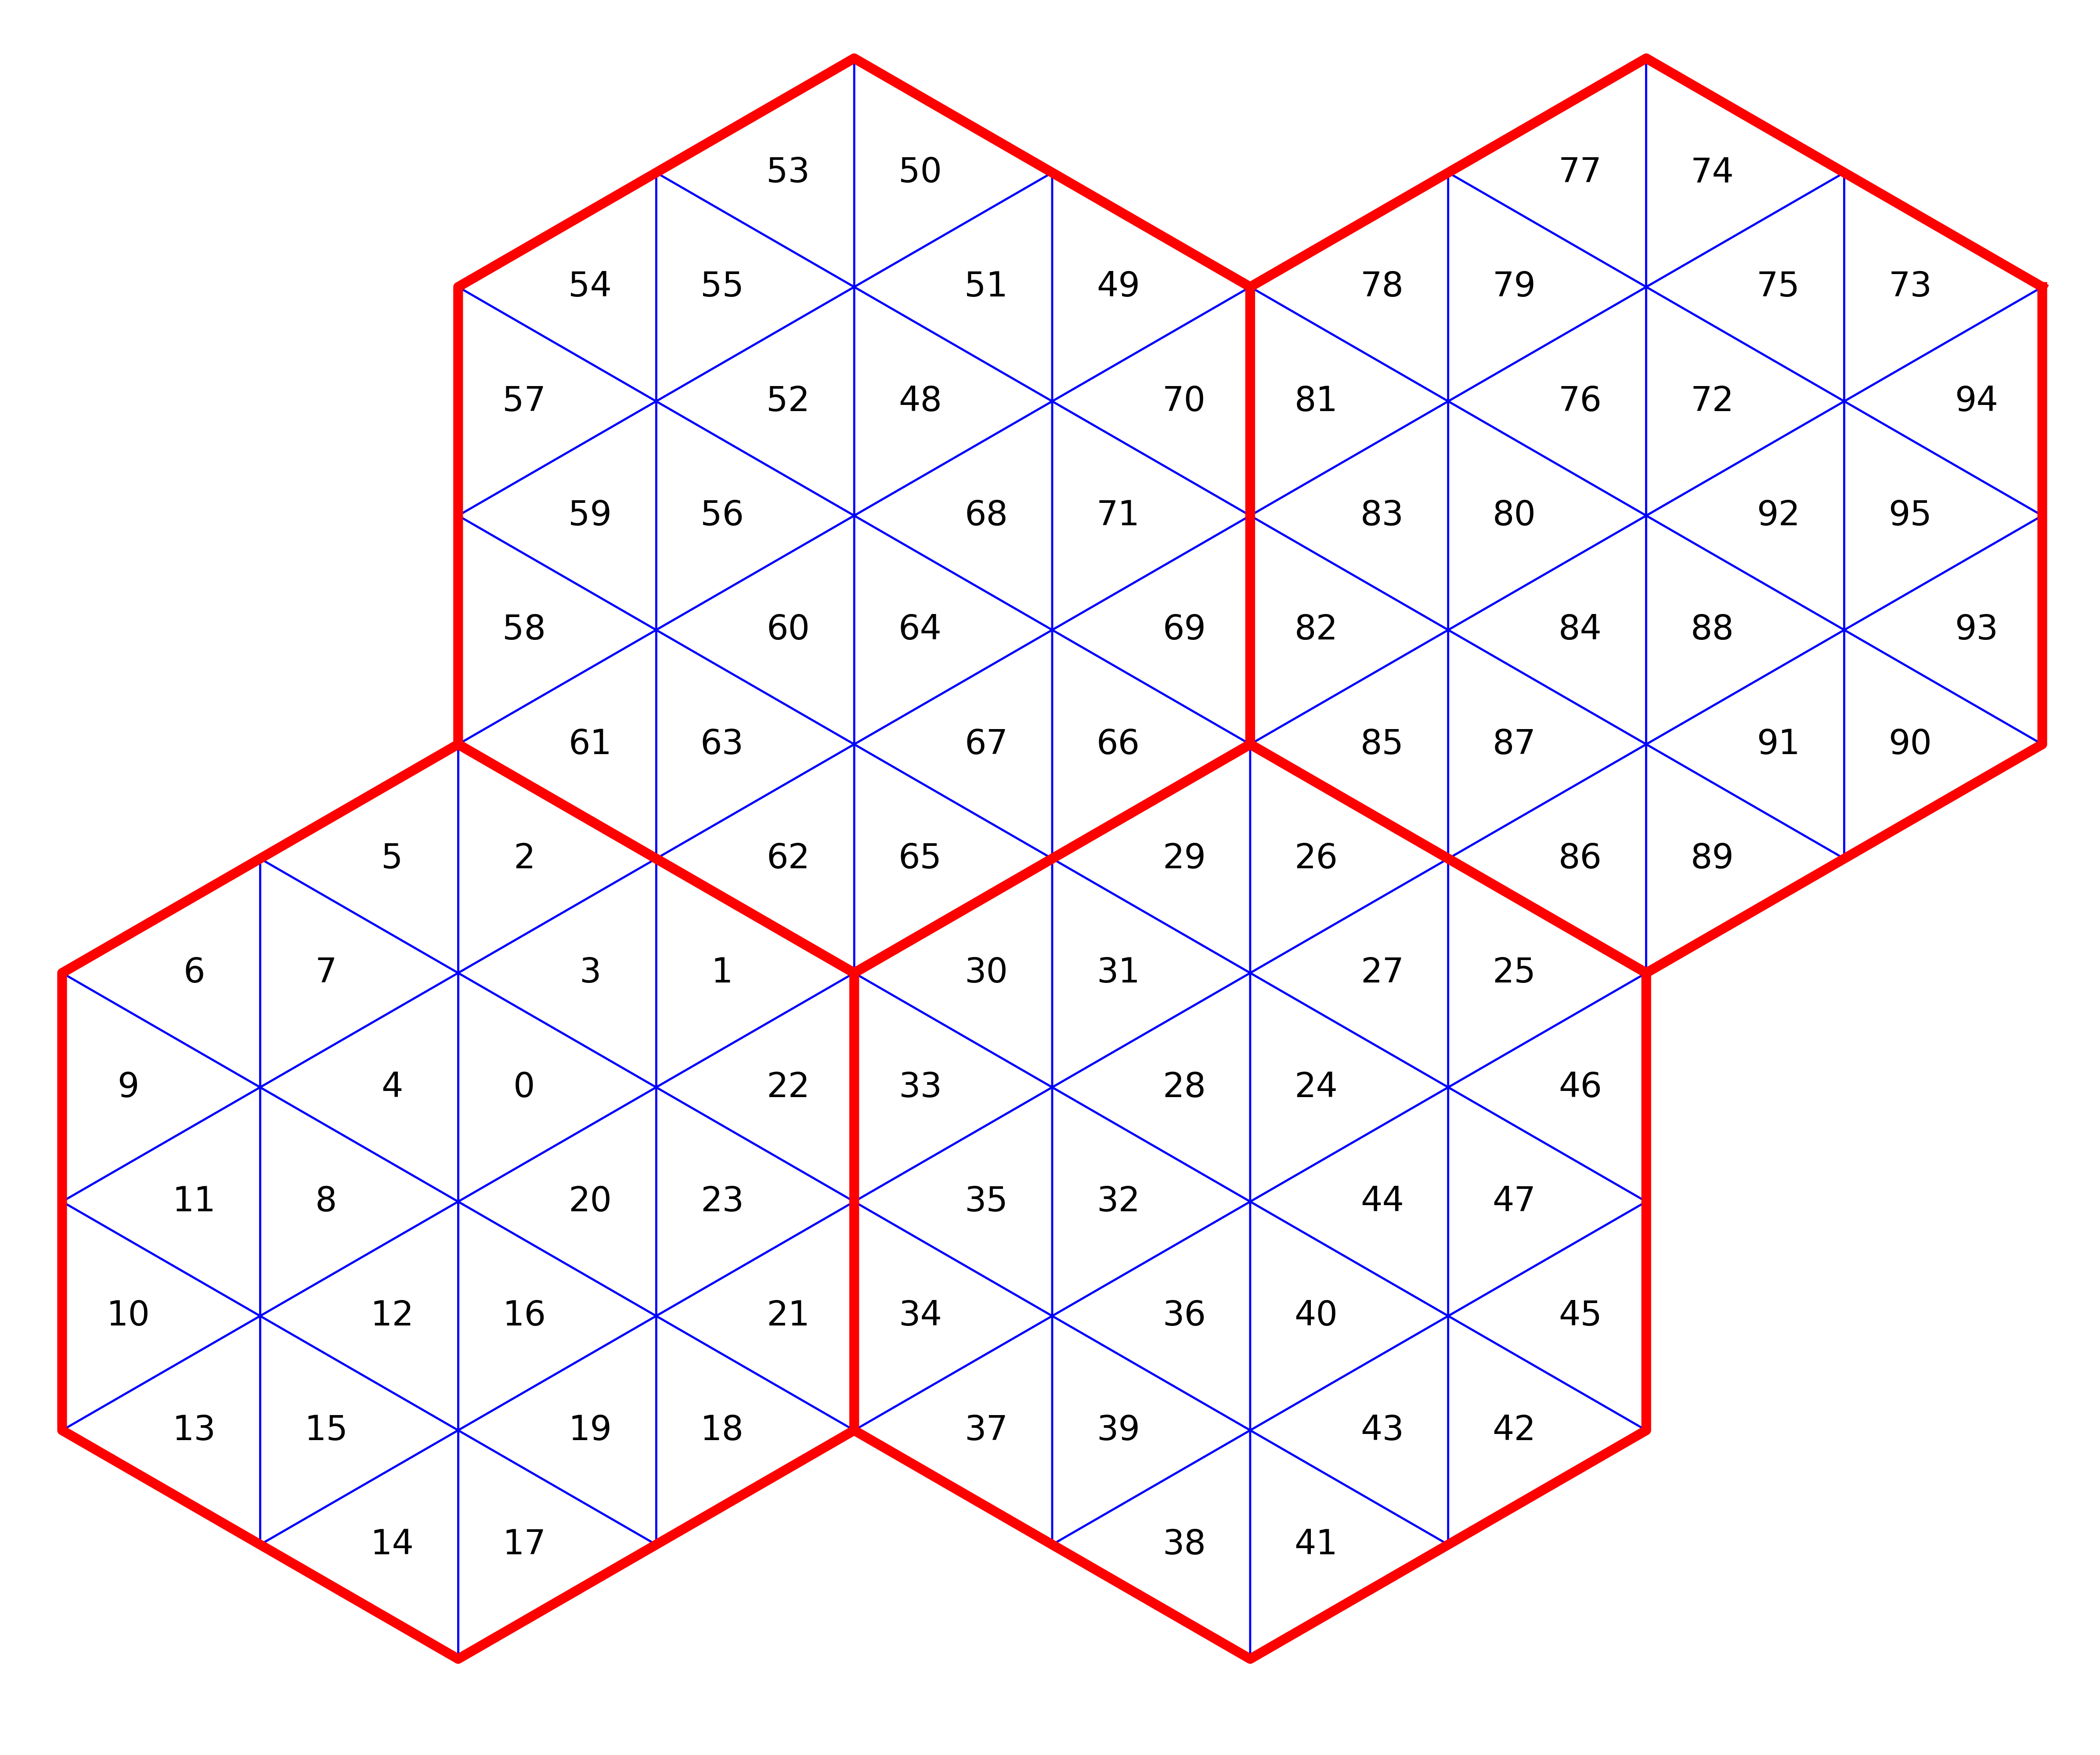
\includegraphics[width=\linewidth]{figures/trial_triangulation_new.png}
        \end{subfigure}
        \caption{2D triangular discretization (left) and hexagon indexing for level 1 (right)}
        \label{fig:2DTri discretization}
\end{figure}
\begin{figure}[H]
        \centering
        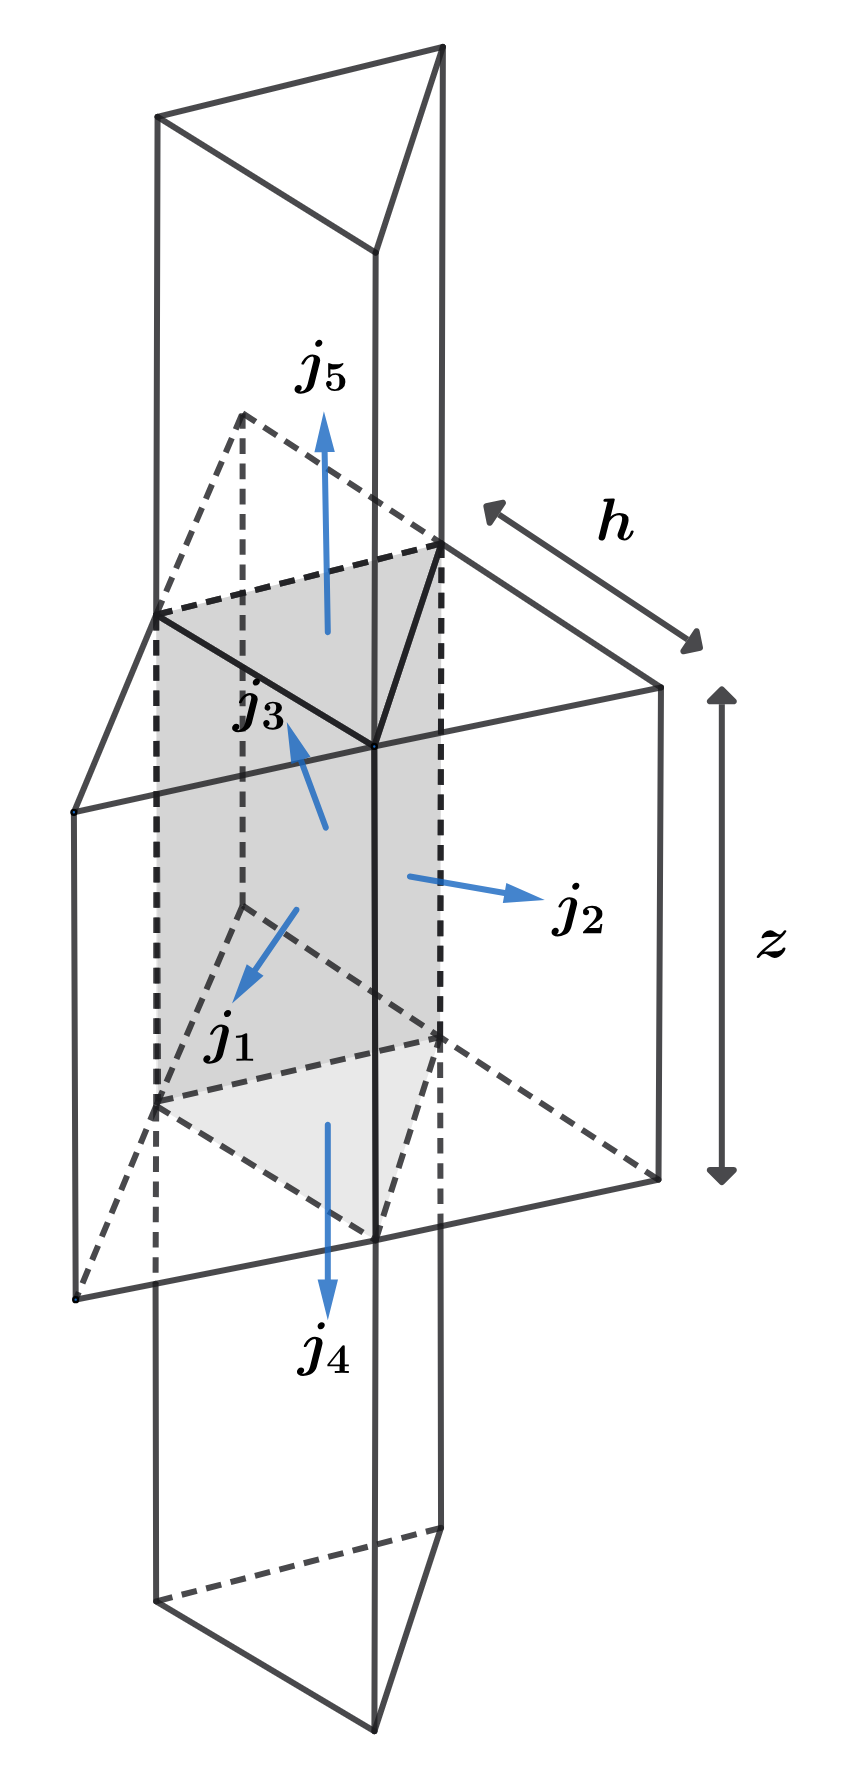
\includegraphics[width=0.35\textwidth]{figures/3DTri_disc2.png}
        \caption{3D discretization of triangular geometries in finite volume method}
        \label{fig:3DTri discretization}
\end{figure}

The discretized form of Eq. \ref{eq:freq_4_ch3} for 3D triangular geometries is as follows:
\begin{equation}
        \begin{aligned}
                \frac{i \omega}{v_g} \delta \phi_{g,i} (\omega) &+ \biggl( \frac{8}{h^2} \biggl( \frac{D_{g,i}D_{g,j1}}{D_{g,i}+D_{g,j1}} + \frac{D_{g,i}D_{g,j2}}{D_{g,i}+D_{g,j2}} + \frac{D_{g,i}D_{g,j3}}{D_{g,i}+D_{g,j3}} \biggr) \delta \phi_{g,i}(\omega) +\\ 
                &\biggl(-\frac{8}{h^2}\frac{D_{g,i}D_{g,j1}}{D_{g,i}+D_{g,j1}}\biggr) \delta \phi_{g,j1}(\omega) + \biggl(-\frac{8}{h^2}\frac{D_{g,i}D_{g,j2}}{D_{g,i}+D_{g,j2}}\biggr) \delta \phi_{g,j2}(\omega) + \biggl(-\frac{8}{h^2}\frac{D_{g,i}D_{g,j3}}{D_{g,i}+D_{g,j3}}\biggr) \delta \phi_{g,j3}(\omega) \biggr) + \\ 
                &\frac{1}{(\Delta z)^2} \biggl( -\frac{2D_{g,i}D_{g,j4}}{D_{g,i}+D_{g,j4}} \delta \phi_{g,j4}(\omega) + \biggl(\frac{2D_{g,i}D_{g,j4}}{D_{g,i}+D_{g,j4}}+\frac{2D_{g,i}D_{g,j5}}{D_{g,i}+D_{g,j5}}\biggr) \delta \phi_{g,i}(\omega) - \\
                &\frac{2D_{g,i}D_{g,j5}}{D_{g,i}+D_{g,j5}} \delta \phi_{g,j5}(\omega) \biggr) + \Sigma_{t,g,i} \delta \phi_{g,i}(\omega) - \sum_{g' = 1}^{G} \biggl(\Sigma_{s0,g',g,i} \delta \phi_{g',i}(\omega) \biggr) - \\
                &\frac{1}{k_{\text{eff}}} \biggl( \chi^p_g (1-\beta_{\text{eff}}) + \chi^d_g \frac{\lambda \beta_{\text{eff}}}{i \omega + \lambda} \biggr)  \biggl(\sum_{g' = 1}^{G} \nu \Sigma_{f,g',i} \delta \phi_{g',i}(\omega) \biggr)= - \delta \Sigma_{t,g,i}(\omega) \phi_{g,i} + \\
                &\sum_{g' = 1}^{G} \biggl(\delta \Sigma_{s0,g',g,i}(\omega) \phi_{g',i}) \biggr) + \frac{1}{k_{\text{eff}}} \biggl( \chi^p_g (1-\beta_{\text{eff}}) + \chi^d_g \frac{\lambda \beta_{\text{eff}}}{i \omega + \lambda} \biggr)  \biggl( \sum_{g' = 1}^{G} \delta \nu \Sigma_{f,g',i}(\omega) \phi_{g',i}) \biggr)
        \end{aligned}
        \label{eq:noise_3D_tri_disc}
\end{equation}

For Eq. \ref{eq:forward_eq_ch3}, the discretization for 3D triangular geometries is as follows:
\begin{equation}
        \begin{aligned}
                \biggl( \frac{8}{h^2} &\biggl( \frac{D_{g,i}D_{g,j1}}{D_{g,i}+D_{g,j1}} + \frac{D_{g,i}D_{g,j2}}{D_{g,i}+D_{g,j2}} + \frac{D_{g,i}D_{g,j3}}{D_{g,i}+D_{g,j3}} \biggr) \phi_{g,i} + \biggl(-\frac{8}{h^2}\frac{D_{g,i}D_{g,j1}}{D_{g,i}+D_{g,j1}}\biggr) \phi_{g,j1} + \\ 
               &\biggl(-\frac{8}{h^2}\frac{D_{g,i}D_{g,j2}}{D_{g,i}+D_{g,j2}}\biggr) \phi_{g,j2} + \biggl(-\frac{8}{h^2}\frac{D_{g,i}D_{g,j3}}{D_{g,i}+D_{g,j3}}\biggr) \phi_{g,j3} \biggr) + \\ 
                &\frac{1}{(\Delta z)^2} \biggl( -\frac{2D_{g,i}D_{g,j4}}{D_{g,i}+D_{g,j4}} \phi_{g,j4} + \biggl(\frac{2D_{g,i}D_{g,j4}}{D_{g,i}+D_{g,j4}}+\frac{2D_{g,i}D_{g,j5}}{D_{g,i}+D_{g,j5}}\biggr) \phi_{g,i} - \\
                &\frac{2D_{g,i}D_{g,j5}}{D_{g,i}+D_{g,j5}} \phi_{g,j5} \biggr) + \Sigma_{t,g,i} \phi_{g,i} =  \sum_{g' = 1}^{G} \biggl(\Sigma_{s0,g',g,i} \phi_{g',i}) \biggr)\\
                & + \frac{1}{k_{\text{eff}}} \biggl( \chi^p_g (1-\beta_{\text{eff}}) + \chi^d_g \frac{\lambda \beta_{\text{eff}}}{i \omega + \lambda} \biggr)  \biggl( \sum_{g' = 1}^{G} \nu \Sigma_{f,g',i} \phi_{g',i}) \biggr)
        \end{aligned}
        \label{eq:forward_3D_tri_disc}
\end{equation}

For Eq. \ref{eq:adjoint_eq_ch3}, the discretization for 3D triangular geometries is as follows:
\begin{equation}
        \begin{aligned}
                \biggl( \frac{8}{h^2} &\biggl( \frac{D_{g,i}D_{g,j1}}{D_{g,i}+D_{g,j1}} + \frac{D_{g,i}D_{g,j2}}{D_{g,i}+D_{g,j2}} + \frac{D_{g,i}D_{g,j3}}{D_{g,i}+D_{g,j3}} \biggr) \phi_{g,i}^{\dagger} + \biggl(-\frac{8}{h^2}\frac{D_{g,i}D_{g,j1}}{D_{g,i}+D_{g,j1}}\biggr) \phi_{g,j1}^{\dagger} + \\ 
               &\biggl(-\frac{8}{h^2}\frac{D_{g,i}D_{g,j2}}{D_{g,i}+D_{g,j2}}\biggr) \phi_{g,j2}^{\dagger} + \biggl(-\frac{8}{h^2}\frac{D_{g,i}D_{g,j3}}{D_{g,i}+D_{g,j3}}\biggr) \phi_{g,j3}^{\dagger} \biggr) + \\ 
                &\frac{1}{(\Delta z)^2} \biggl( -\frac{2D_{g,i}D_{g,j4}}{D_{g,i}+D_{g,j4}} \phi_{g,j4}^{\dagger} + \biggl(\frac{2D_{g,i}D_{g,j4}}{D_{g,i}+D_{g,j4}}+\frac{2D_{g,i}D_{g,j5}}{D_{g,i}+D_{g,j5}}\biggr) \phi_{g,i}^{\dagger} - \\
                &\frac{2D_{g,i}D_{g,j5}}{D_{g,i}+D_{g,j5}} \phi_{g,j5}^{\dagger} \biggr) + \Sigma_{t,g,i} \phi_{g,i}^{\dagger} =  \\
                &\sum_{g' = 1}^{G} \biggl(\Sigma_{s0,g,g',i} \phi_{g',i}^{\dagger} \biggr) + \frac{1}{k_{\text{eff}}} \nu \Sigma_{f,g,i} \biggl( \sum_{g' = 1}^{G} \biggl( \chi^p_{g'} (1-\beta_{\text{eff}}) + \chi^d_{g'} \frac{\lambda \beta_{\text{eff}}}{i \omega + \lambda} \biggr) \phi_{g',i}^{\dagger} \biggr)
        \end{aligned}
        \label{eq:adjoint_3D_tri_disc}
\end{equation}

\subsection{Boundary Conditions}

The boundary conditions implemented here are vacuum, reflective, and zero flux. The vacuum boundary condition is defined as follows,
\begin{equation}
    J_{-}(\textbf{r}_b) = \frac{\phi(\textbf{r}_b)}{4} + \frac{1}{2}D(\textbf{r}_b) \nabla \phi(\textbf{r}_b) = 0
\end{equation}
The reflective boundary condition is defined as follows,
\begin{equation}
    D(\textbf{r}_b) \nabla \phi(\textbf{r}_b) = 0
\end{equation}
For the implementation in the developed tool, the albedo boundary condition is used. The definition of the albedo boundary condition is as follows:
\begin{equation}\label{eq:define_albedo}
    \frac{J_{-}(\textbf{r}_b)}{J_{+}(\textbf{r}_b)} = \alpha
\end{equation}
where $\alpha$ has a range of values between 0 and 1. We can derive Eq. \ref{eq:define_albedo} further as follows:
\begin{equation}
    \begin{aligned}
        J_{-}(\textbf{r}_b) &= \alpha J_{+}(\textbf{r}_b)\\
        \frac{\phi(\textbf{r}_b)}{4} + \frac{1}{2} D(\textbf{r}_b) \nabla \phi(\textbf{r}_b) &= \alpha \biggl( \frac{\phi(\textbf{r}_b)}{4} - \frac{1}{2} D(\textbf{r}_b) \nabla \phi(\textbf{r}_b) \biggr) \\
        (1-\alpha) \frac{\phi(\textbf{r}_b)}{4} + (1+\alpha) \biggl( \frac{1}{2} D(\textbf{r}_b) \nabla \phi(\textbf{r}_b) \biggr) &= 0  \\
        \frac{1-\alpha}{1+\alpha} \frac{\phi(\textbf{r}_b)}{4} + \frac{1}{2} D(\textbf{r}_b) \nabla \phi(\textbf{r}_b) &= 0
    \end{aligned}
\end{equation}
Albedo is a convenient boundary conditions because $\alpha$ = 0 corresponds to the vacuum boundary condition, $\alpha$ = 1 corresponds to reflective boundary condition. Finally, the zero flux boundary condition is defined as follows,
\begin{equation}
    \phi(\textbf{r}_b) = 0
\end{equation}

\subsection{Numerical Methods}

To solve the forward equation (Eq. \ref{eq:forward_eq_ch3}), adjoint equation (Eq. \ref{eq:adjoint_eq_ch3}), and neutron noise equation (Eq. \ref{eq:freq_4_ch3}), we can write those equations in matrix form as follows:
\begin{equation}\label{eq:matrix_forward}
    A_{\text{fw}} \phi_{\text{fw}} = \frac{1}{k_{\text{eff}}} F_{\text{fw}} \phi_{\text{fw}}
\end{equation}
\begin{equation}\label{eq:matrix_adjoint}
    A^{\dagger} \phi^{\dagger} = \frac{1}{k_{\text{eff}}} F^{\dagger} \phi^{\dagger}
\end{equation}
\begin{equation}\label{eq:matrix_noise}
    A_{\text{noise}} \delta \phi_{\text{noise}} = S_{\text{noise}}
\end{equation}
where Eq. \ref{eq:matrix_forward} is the matrix form of forward equation, Eq. \ref{eq:matrix_adjoint} is the matrix from of adjoint equation, and equation \ref{eq:matrix_noise} is the matrix form of neutron noise equation.

In Eq. \ref{eq:matrix_forward}-\ref{eq:matrix_noise}, the coefficient matrices (e.g. $A_{\text{fw}}$, $A^{\dagger}$, and $A_{\text{noise}}$) are large, sparse, and banded. The size of these coefficients is ($\text{G} * N \times \text{G} * N$), where G is the number of neutron energy groups and N is the spatial grid of the system of interest. In this tool, the geometries are discretized using a uniform mesh. Coefficient matrices are constructed using sparse array format. The terms such as $D$, $\Sigma_t$,$\Sigma_s$, and $\nu \Sigma_f$ are constructed separately. Then, the operators are combined into the coefficient matrices. 

Since we are solving a sparse system of equations in Eqs. \ref{eq:matrix_forward}-\ref{eq:matrix_noise}, it is beneficial to use a sparse matrix solver. In this tool, the sparse matrix solver is obtained from the PETSc (Portable, Extensible Toolkit for Scientific Computation) Library. PETSc is a suite of algorithms and data structures for the solution of problems arising in scientific and engineering applications, especially those modeled by partial differential equation, and targeted for high performance parallel computing environments \cite{dalcinParallelDistributedComputing2011}. PETSc includes a large suite of scalable parallel linear and nonlinear equation solvers, ODE integrators, and optimization algorithms for application codes written in C, C++, Fortran, and Python \cite{balayPETScTAOUsers2025}.

The matrix solver in this tool is divided into two categories, the eigenvalue solver and fixed source solver. The eigenvalue solver is used to solve forward and adjoint equations, while the fixed source solver is used to solve the neutron noise equation. For all the matrix solvers, the tool applies the iterative Generalized Minimal Residual (GMRES) method. The acceleration of the convergence is obtained from a preconditioner, which can be chosen between Incomplete LU (ILU) and LU preconditioner. The eigenvalue problem is solved using the standard power iteration method, while the fixed source problem is solved with a conventional linear system solver.

\section{Simulated Cases for Verification Purposes}
\label{sec:simulated_vandv}

\subsection{2D Homogeneous Reactor}

In this case, simulations were performed and compared with the analytical solutions based on an infinitely long homogeneous cylindrical reactor with radius 150 cm. For the simulations, the cylinder is approximated using triangular meshes. There are 19,692 triangular meshes in this case. A vacuum boundary condition is assumed on all sides of the reactor. The homogeneous macroscopic cross-sections, the diffusion coefficients, and the kinetic parameters are given in Table \ref{table:2DHomogParam}. 

\begin{table}[H]
\centering
\caption{Kinetic parameters and cross-sections of 2D Homogeneous Reactor in Triangular Grid}
\label{table:2DHomogParam}

% Define custom color
\definecolor{myyellow}{RGB}{255, 255, 150}

\renewcommand{\arraystretch}{1.0} % row height

\begin{tabular}{|>{\centering\arraybackslash}m{3cm}|>{\centering\arraybackslash}m{3cm}|>{\centering\arraybackslash}m{3cm}|}
\hline
\textbf{Parameter} & \textbf{Value} & \textbf{Unit} \\ \hline
\rowcolor{myyellow}\multicolumn{3}{|c|}{\textbf{Kinetic Parameters}} \\ \hline
$\beta_{\text{eff}}$ & 535 & pcm \\ \hline
$\lambda$ & 0.085 & $s^{-1}$ \\ \hline
$v_1$ & 18372300 & cm/s \\ \hline
$v_2$ & 413086 & cm/s \\ \hline

\rowcolor{myyellow}\multicolumn{3}{|c|}{\textbf{Cross-sections}} \\ \hline
$\Sigma_{a,1} $ & 0.0115 & $cm^{-1}$ \\ \hline
$\Sigma_{a,2} $ & 0.1019 & $cm^{-1}$ \\ \hline
$\nu \Sigma_{f,1} $ & 0.0057 & $cm^{-1}$ \\ \hline
$\nu \Sigma_{f,2} $ & 0.14425 & $cm^{-1}$ \\ \hline
$\Sigma_{R} $ & 0.0151 & $cm^{-1}$ \\ \hline
$D_1$ & 0.5376 & cm \\ \hline
$D_2$ & 0.1423 & cm \\ \hline

\end{tabular}
\end{table}

\subsubsection{Forward Flux Solution}

For the forward flux, the analytical solution is described in Eq. \ref{eq:2DHomog_forward_ana}.
\begin{equation}\label{eq:2DHomog_forward_ana}
    \begin{bmatrix}
        \phi_1(r) \\[4pt]
        \phi_2(r)
    \end{bmatrix}
    =
    \begin{bmatrix}
    1 \\[4pt]
    c_\mu
    \end{bmatrix}
    J_0\!\big(B_g r\big)
\end{equation}
where,
\begin{equation}
    \begin{aligned}
        B_g^2 &= \biggl( \frac{j_0}{R + 2D_1} \biggr)^2 \\
        c_{\mu} &= \frac{\Sigma_R}{\Sigma_{a,2} + D_2 B_g^2}
    \end{aligned}
\end{equation}
$j_0$ is the first root of the Bessel function $J_0$.

The analytical $k_{\text{eff}}$ is calculated using Eq. \ref{eq:2DHomog_forward_ana_keff}.
\begin{equation}
    k_{\text{eff}} = \frac{\nu \Sigma_{f,2} \Sigma_R + \nu \Sigma_{f,1} (\Sigma_{a,2} + D_2 B_g^2)}{(\Sigma_{a,1} + D_1 B_g^2 + \Sigma_R) (\Sigma_{a,2} + D_2 B_g^2)}
    \label{eq:2DHomog_forward_ana_keff}
\end{equation}

The comparison between the tool and the analytical solutions are described in Table \ref{table:2DHomog_fw_results} and Figure \ref{fig:2DHomog_fw_results_compare}.

\begin{table}[H]
        \centering
        \caption{Eigenvalue comparison of 2D Homogeneous Reactor}
        \label{table:2DHomog_fw_results}
        \begin{tabular}{ | M{3.5cm} | M{2cm} | } 
         \hline
         $k_{\text{eff}}$ Analytical & 1.01241  \\
         \hline
         $k_{\text{eff}}$ tool & 1.01241  \\
         \hline
         Absolute Error (pcm) & 0.0  \\
         \hline
        \end{tabular}
\end{table}

\begin{figure}[H]
        \centering
        \begin{subfigure}{.48\textwidth}
          \centering
          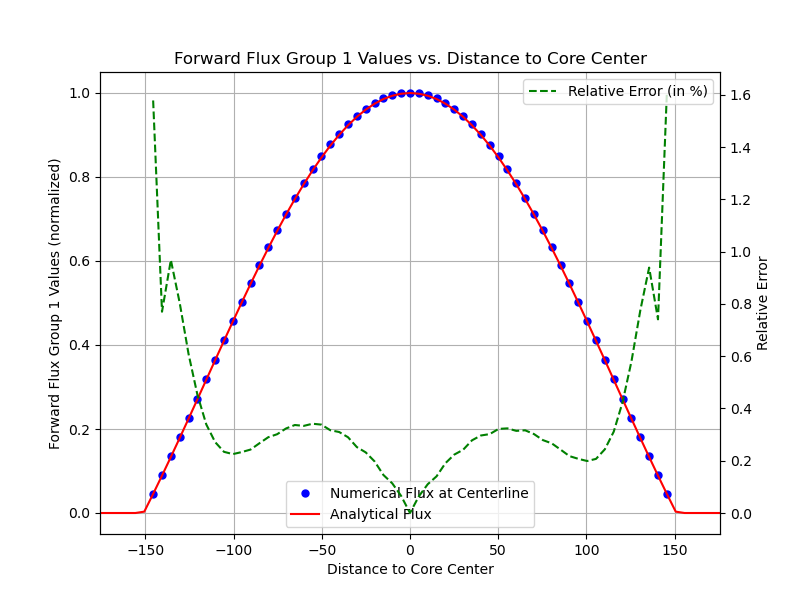
\includegraphics[width=\linewidth]{figures/Verification_PHI_magnitude_G1.png}
        \end{subfigure}
        \hfill
        \begin{subfigure}{.48\textwidth}
          \centering
          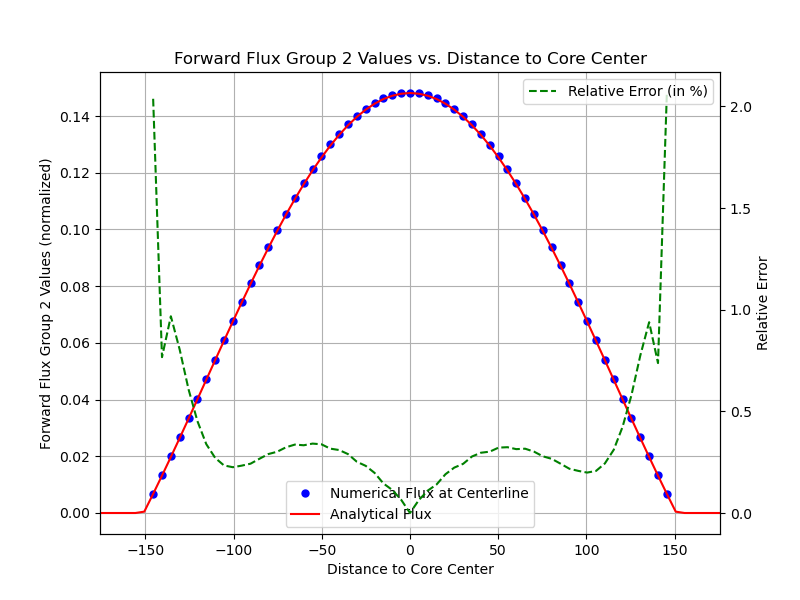
\includegraphics[width=\linewidth]{figures/Verification_PHI_magnitude_G2.png}
        \end{subfigure}
        \caption{Comparison of forward flux at the centerline between the tool and analytical solutions}
        \label{fig:2DHomog_fw_results_compare}
\end{figure}

The results show that the tool agrees well with the analytical solutions of the forward flux, with a maximum error of 2\% at the periphery of the core. The $k_{\text{eff}}$ matches between analytical solution and the developed tool. This demonstrates that the tool performs effectively for 2D triangular geometries.

\subsubsection{Adjoint Flux Solution}

For the adjoint flux, the analytical solution is described in Eq. \ref{eq:2DHomog_adjoint_ana}.
\begin{equation}\label{eq:2DHomog_adjoint_ana}
    \begin{bmatrix}
        \phi_1^{\dagger}(r) \\[4pt]
        \phi_2^{\dagger}(r)
    \end{bmatrix}
    =
    \begin{bmatrix}
    1 \\[4pt]
    c_\mu^{\dagger}
    \end{bmatrix}
    J_0\!\big(B_g r\big)
\end{equation}
where,
\begin{equation}
    \begin{aligned}
        c_{\mu}^{\dagger} &= \frac{1}{k_\text{eff}} \frac{\nu \Sigma_{f,2}}{\Sigma_{a,2} + D_2 B_g^2}
    \end{aligned}
\end{equation}

The comparison between the tool and the analytical solutions are described in Figure \ref{fig:2DHomog_adj_results_compare}.

\begin{figure}[H]
        \centering
        \begin{subfigure}{.48\textwidth}
          \centering
          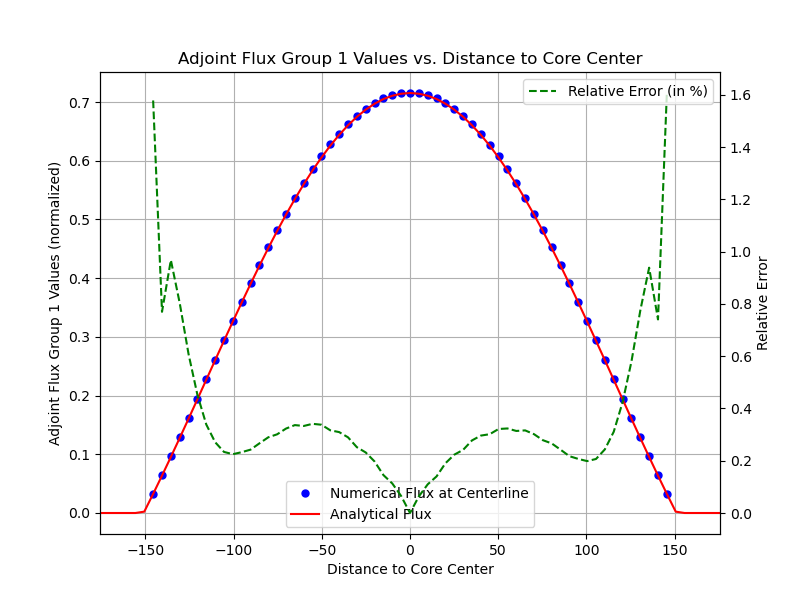
\includegraphics[width=\linewidth]{figures/Verification_PHI_ADJ_magnitude_G1.png}
        \end{subfigure}
        \hfill
        \begin{subfigure}{.48\textwidth}
          \centering
          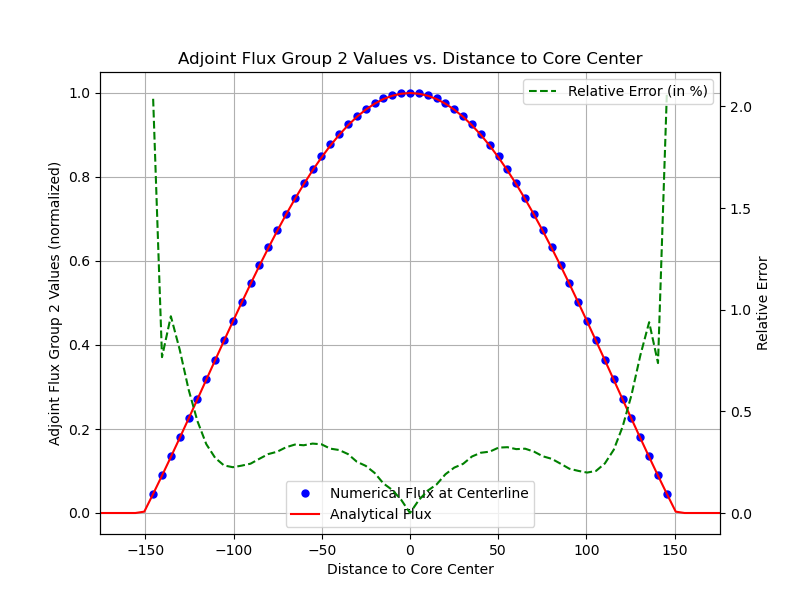
\includegraphics[width=\linewidth]{figures/Verification_PHI_ADJ_magnitude_G2.png}
        \end{subfigure}
        \caption{Comparison of adjoint flux at the centerline between the tool and analytical solutions}
        \label{fig:2DHomog_adj_results_compare}
\end{figure}

The results show that the tool agrees well with the analytical solutions of the adjoint flux, with a maximum error of 2\% at the periphery of the core. This indicates that the tool performs effectively for 2D triangular geometries.

\subsubsection{Neutron Noise Solution}

In this case, it is defined that the noise source perturbed the absorption cross-section.
\begin{equation}
    \delta \Sigma_{a,2}(\textbf{r}_p,\omega) = 0.3
\end{equation}

where we define $\textbf{r}_p$ at the center of the core with a frequency of 1 Hz. The analytical solutio for this problem is described in Eq. \ref{eq:2DHomog_noise_ana}.
\begin{equation}\label{eq:2DHomog_noise_ana}
    \begin{bmatrix}
       \delta \phi_1(r, \omega) \\[4pt]
       \delta \phi_2(r, \omega)
    \end{bmatrix}
    = \frac{1}{4 D_2(c_\lambda - c_\mu)}
    \begin{bmatrix}
        1 \\[4pt]
        c_\mu
    \end{bmatrix}
    \biggl(J_0(\mu r) \frac{Y_0(\mu R)}{J_0(\mu R)} - Y_0(\mu r) \biggr) - \frac{1}{2 \pi D_2(c_\lambda - c_\mu)}
    \begin{bmatrix}
        1 \\[4pt]
        c_\lambda
    \end{bmatrix}
    \biggl(K_0(\lambda r) - I_0(\lambda r) \frac{K_0(\lambda R)}{I_0(\lambda R)} \biggr) 
\end{equation}
where,
\begin{equation}
    \begin{aligned}
        \mu^2 &= \frac{-(\Sigma_1 D_2 + \Sigma_2 D_1) + \sqrt{(\Sigma_1 D_2 + \Sigma_2 D_1)^2 -4 D_1 D_2 (\Sigma_1 \Sigma_2 - \Sigma_R \nu \Sigma_{f,2}}}{2 D_1 D_2} \\
        \lambda^2 &= \frac{(\Sigma_1 D_2 + \Sigma_2 D_1) + \sqrt{(\Sigma_1 D_2 + \Sigma_2 D_1)^2 -4 D_1 D_2 (\Sigma_1 \Sigma_2 - \Sigma_R \nu \Sigma_{f,2}}}{2 D_1 D_2} \\
        c_\mu &= \frac{\Sigma_R}{\Sigma_2 + D_2 \mu^2} \\
        c_\lambda &= \frac{\Sigma_R}{\Sigma_2 - D_2 \lambda^2} \\
        \Sigma_1 &= \Sigma_{a,1} + \frac{i\omega}{v_1} + \Sigma_R - \nu \Sigma_{f,1} \\
        \Sigma_2 &= \Sigma_{a,2} + \frac{i\omega}{v_2}
    \end{aligned}
\end{equation}

The comparison between the developed tool and analytical solutions are described in Figure \ref{fig:2DHomog_noise_results_diff_phi}

\begin{figure}[H]
        \centering
        \begin{subfigure}{.48\textwidth}
          \centering
          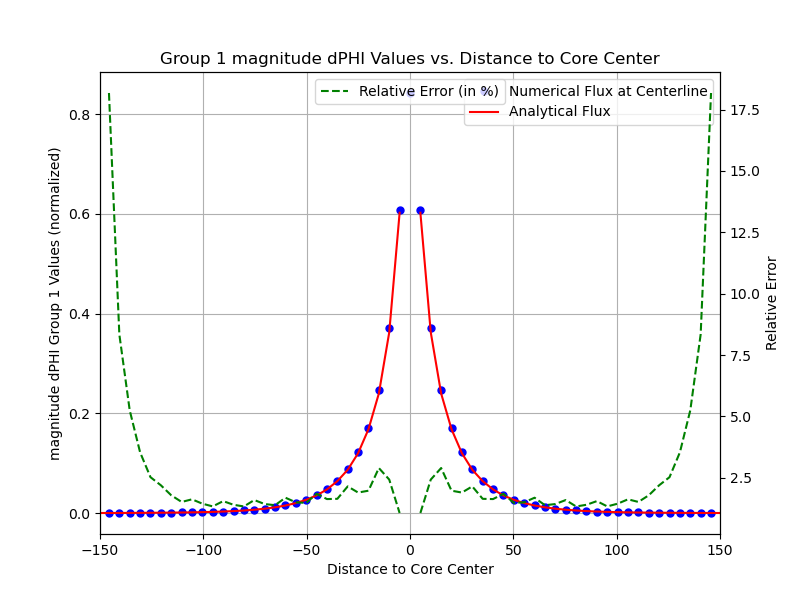
\includegraphics[width=\linewidth]{figures/Verification_dPHI_magnitude_G1.png}
        \end{subfigure}
        \hfill
        \begin{subfigure}{.48\textwidth}
          \centering
          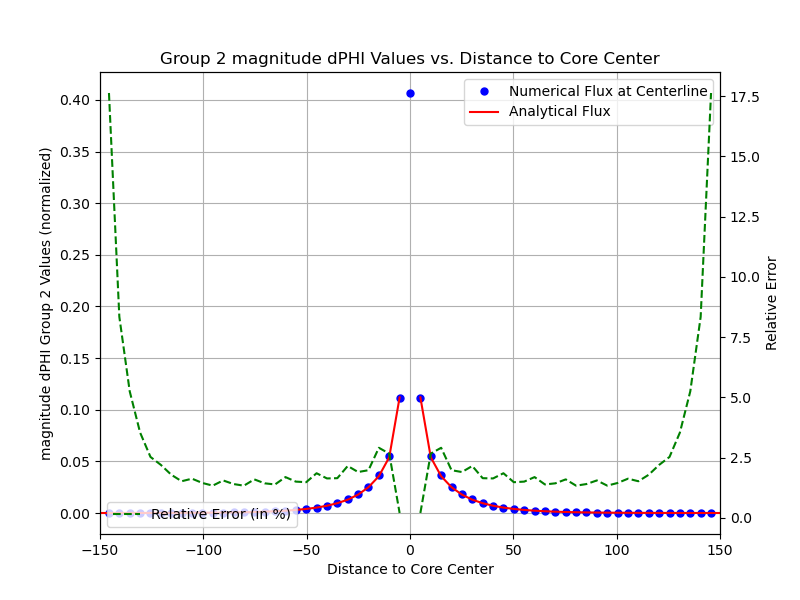
\includegraphics[width=\linewidth]{figures/Verification_dPHI_magnitude_G2.png}
        \end{subfigure}
\end{figure}
\begin{figure}[H]\ContinuedFloat
        \centering
        \begin{subfigure}{.48\textwidth}
          \centering
          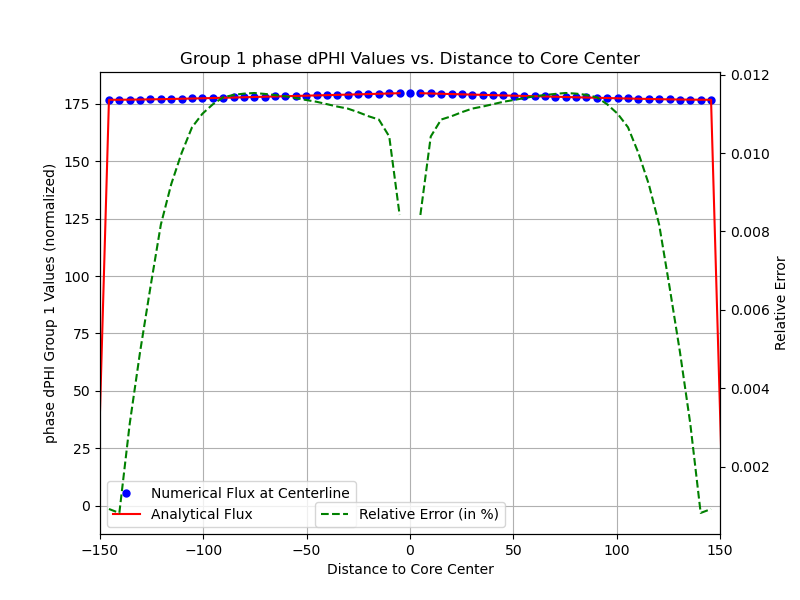
\includegraphics[width=\linewidth]{figures/Verification_dPHI_phase_G1.png}
        \end{subfigure}
        \hfill
        \begin{subfigure}{.48\textwidth}
          \centering
          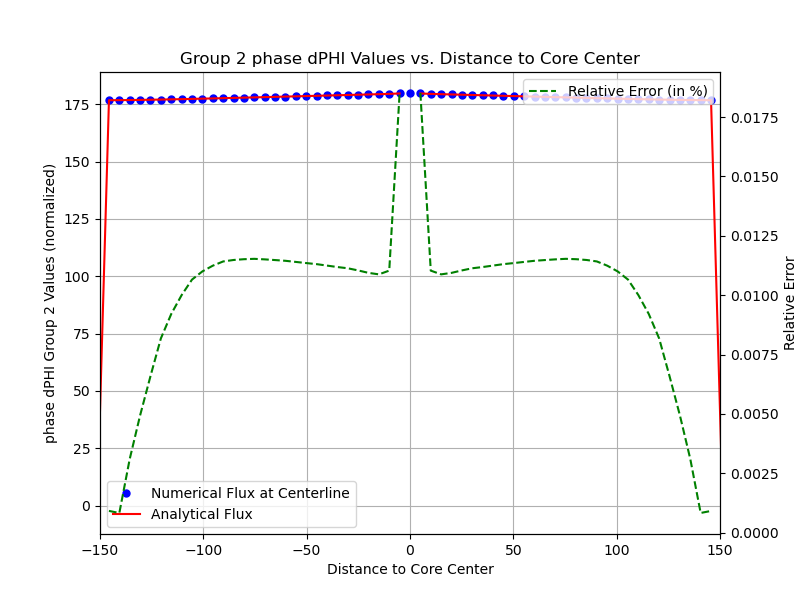
\includegraphics[width=\linewidth]{figures/Verification_dPHI_phase_G2.png}
        \end{subfigure}
        \caption{Comparison of neutron noise at the centerline between the developed tool and analytical solutions}
        \label{fig:2DHomog_noise_results_diff_phi}
\end{figure}

The results show that the solutions for both magnitude and phase in each group agree well with the analytical solution. Since the noise source is defined as perturbations in $\Sigma_{a,2}$, the noise in group 2 reaches its peak at the center of the core. The relative error is higher in the periphery, which is similar to previous cases, due to the neutron noise value being close to zero but still within a reasonable range. Overall, the tool works well compared to the analytical solutions.

\subsection{2D VVER-400 Benchmark}

The VVER-400 Benchmark is developed from \cite{chaoConformalMappingHexagonal1995} to simulate the capability for hexagonal geometries. The VVER-440-type reactor core design features large control rod assemblies that do not contain fuel rods. As a control rod assembly moves into the core, it pushes the fuel assembly underneath out of the way. This results in a significant flux gradient near the interfaces of the control rod assembly and its neighboring fuel assemblies. The core consists of 312 standard fuel assemblies, 37 control assemblies, and a layer of reflector assemblies surrounding the core boundary. The fuel assembly pitch is 14.7 cm. A vacuum boundary condition was applied to the outer boundary of the reflector. In this section, the forward flux is simulated and compared with FEMFFUSION, a finite element-based code developed by Universitat Politècnica de València \cite{vidal-ferrandizFEMFFUSIONFiniteElement2023}. To calculate the error, the normalized power in each assembly is used as the parameter to compare \cite{vidal-ferrandizMovingMeshesSolve2016}. To calculate the normalized power in each assembly, first we define the power for each mesh point $i$ ($P_i$) as follows:
\begin{equation}
    P_i = E_R \sum_g \Sigma_{f,i,g} \phi_{i,g} V_i
\end{equation}
where $E_R$ is the recoverable energy per fission, which is assumed to be constant, and $V_i$ is the volume of the mesh. Then, the normalized power for each assembly $k$ ($P_k$) is defined as follows:
\begin{equation}
    P_k = \frac{\sum_{i=1}^I P_i}{V_k}
\end{equation}
where $I$ is the number of mesh points in one assembly, and $V_k$ is the volume of the assembly. The relative error is calculated as follows:
\begin{equation}
    \varepsilon_k = \frac{|P_{k, \text{calc}}-P_{k, \text{ref}}|}{|P_{k, \text{ref}}|}
\end{equation}

\subsubsection{Forward Flux Solution}

For the tool, the hexagon is divided into six triangular mesh. The eigenvalue comparison is in Table \ref{table:2DVVER_fw_results}, while forward flux and the forward flux comparison to FEMFFUSION are in Figure \ref{fig:2DVVER_fw_results_flx} - \ref{fig:2DVVER_fw_results_diff_phi}.

\begin{table}[H]
        \centering
        \caption{Eigenvalue comparison of 2D VVER-400}
        \label{table:2DVVER_fw_results}
        \begin{tabular}{ | M{3.5cm} | M{2cm} | } 
         \hline
         $k_{\text{eff}}$ FEMFFUSION & 1.003495  \\
         \hline
         $k_{\text{eff}}$ tool & 1.002570  \\
         \hline
         Absolute Error (pcm) & 92.5  \\
         \hline
        \end{tabular}
\end{table}

\begin{figure}[H]
        \centering
        \begin{subfigure}{.48\textwidth}
          \centering
          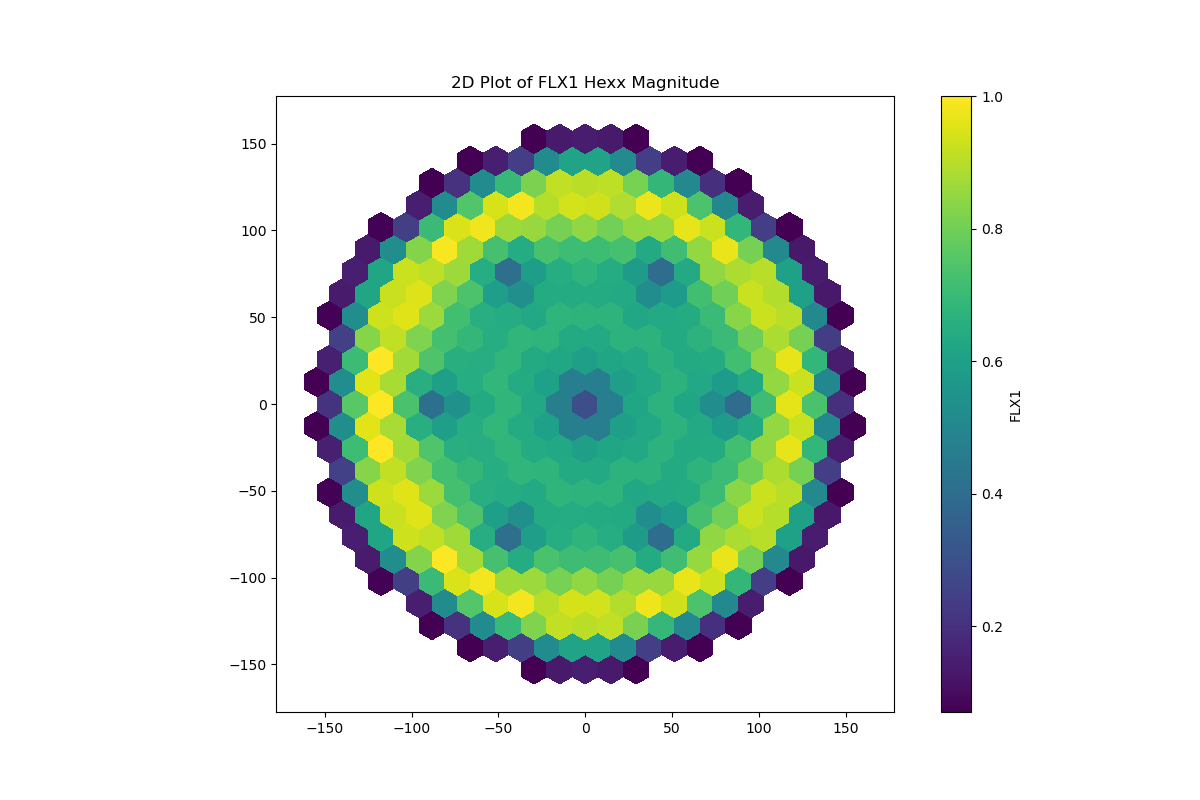
\includegraphics[width=\linewidth]{figures/OBJECTIVES1_TEST05_2DTriMG_VVER400_VandV_level2_FORWARD_FLX_magnitude_G1.png}
        \end{subfigure}
        \hfill
        \begin{subfigure}{.48\textwidth}
          \centering
          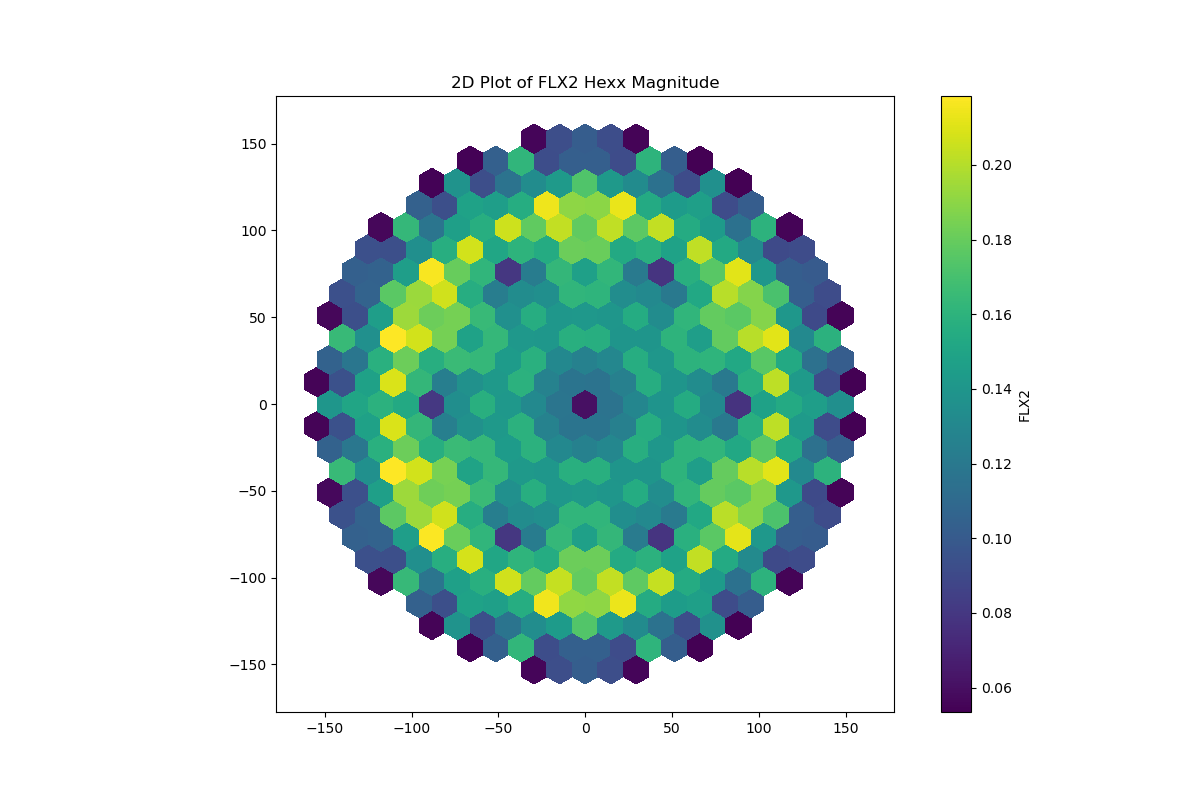
\includegraphics[width=\linewidth]{figures/OBJECTIVES1_TEST05_2DTriMG_VVER400_VandV_level2_FORWARD_FLX_magnitude_G2.png}
        \end{subfigure}
        \caption{Forward flux results from FEMFFUSION}
        \label{fig:2DVVER_fw_results_flx}
\end{figure}
\begin{figure}[H]
        \centering
        \begin{subfigure}{.48\textwidth}
          \centering
          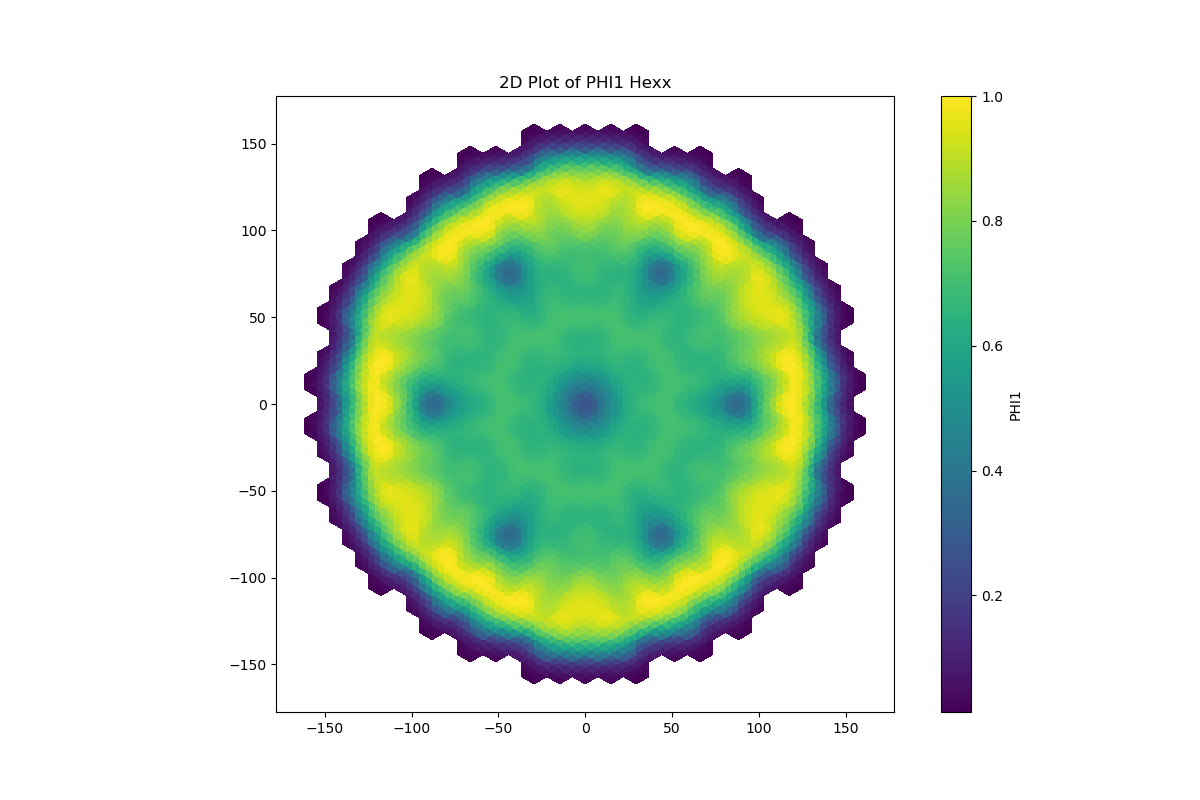
\includegraphics[width=\linewidth]{figures/OBJECTIVES1_TEST05_2DTriMG_VVER400_VandV_level2_FORWARD_PHI_magnitude_G1.png}
        \end{subfigure}
        \hfill
        \begin{subfigure}{.48\textwidth}
          \centering
          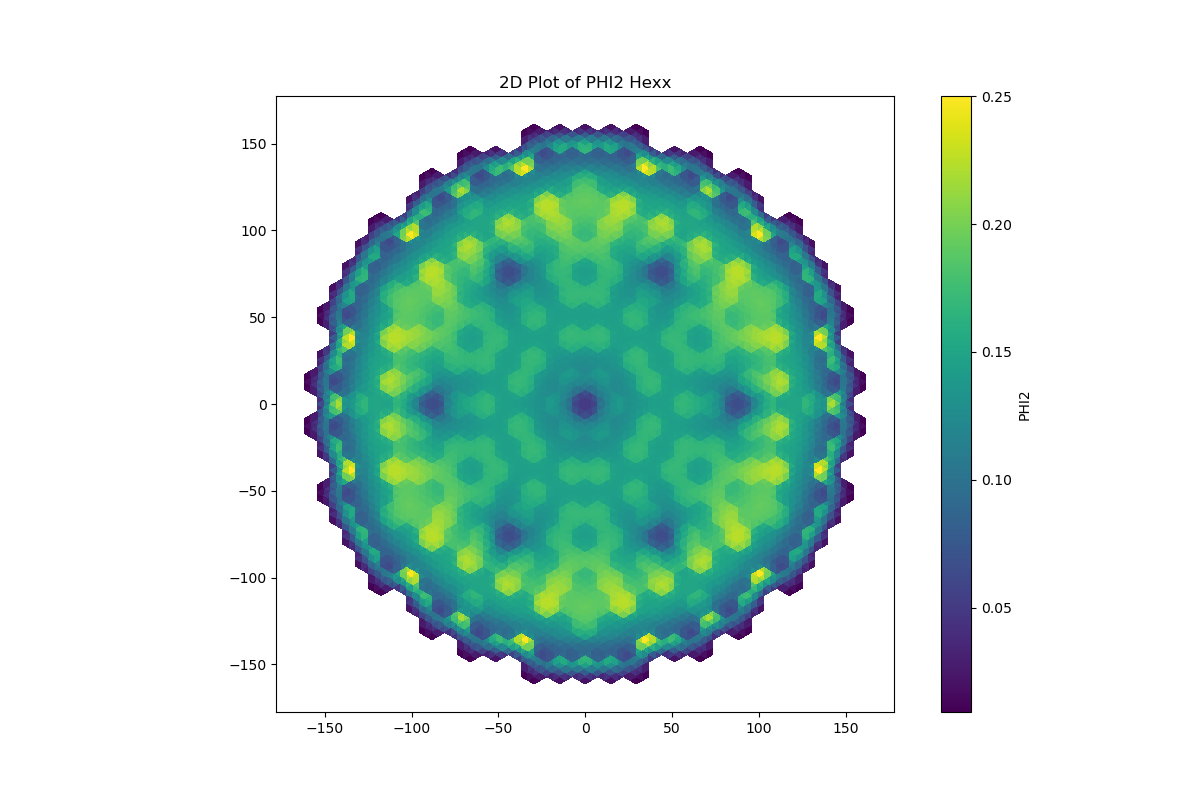
\includegraphics[width=\linewidth]{figures/OBJECTIVES1_TEST05_2DTriMG_VVER400_VandV_level2_FORWARD_PHI_magnitude_G2.png}
        \end{subfigure}
        \caption{Forward flux results from the developed tool}
        \label{fig:2DVVER_fw_results_phi}
\end{figure}
\begin{figure}[H]
        \centering
        \begin{subfigure}{.48\textwidth}
          \centering
          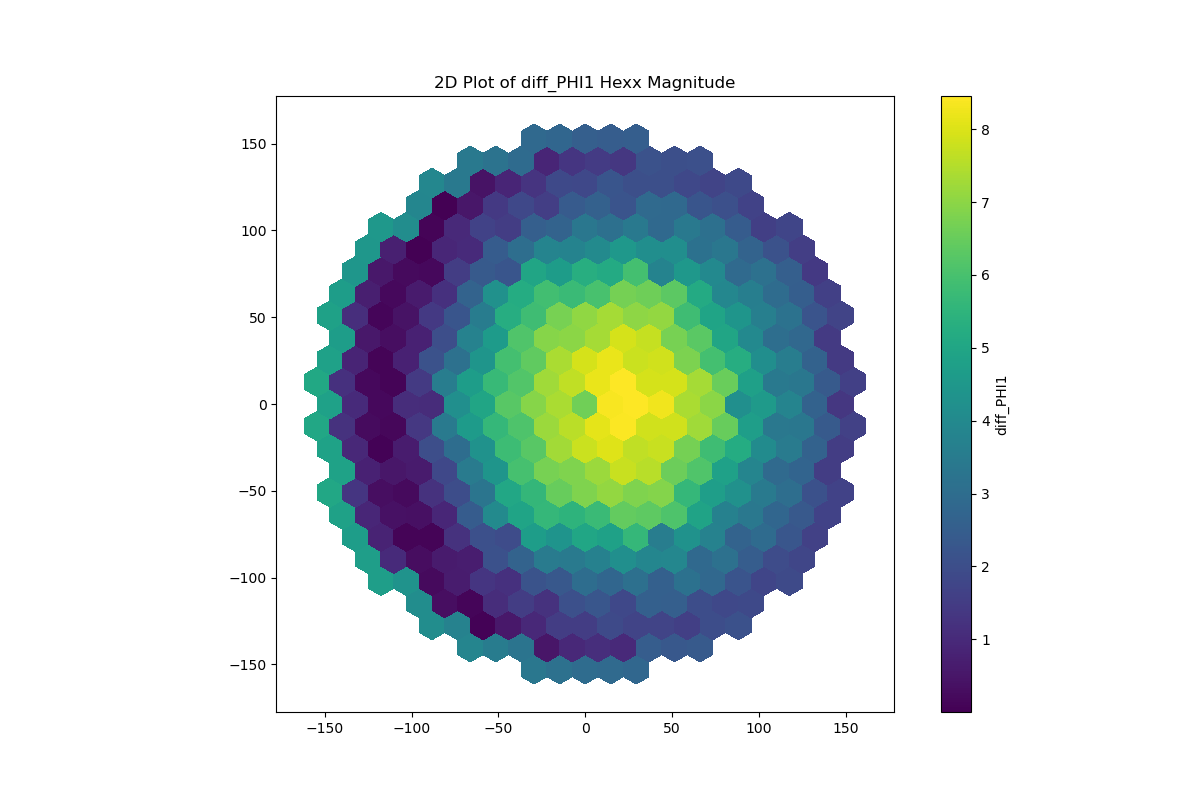
\includegraphics[width=\linewidth]{figures/OBJECTIVES1_TEST05_2DTriMG_VVER400_VandV_level2_FORWARD_diff_PHI_magnitude_G1.png}
        \end{subfigure}
        \hfill
        \begin{subfigure}{.48\textwidth}
          \centering
          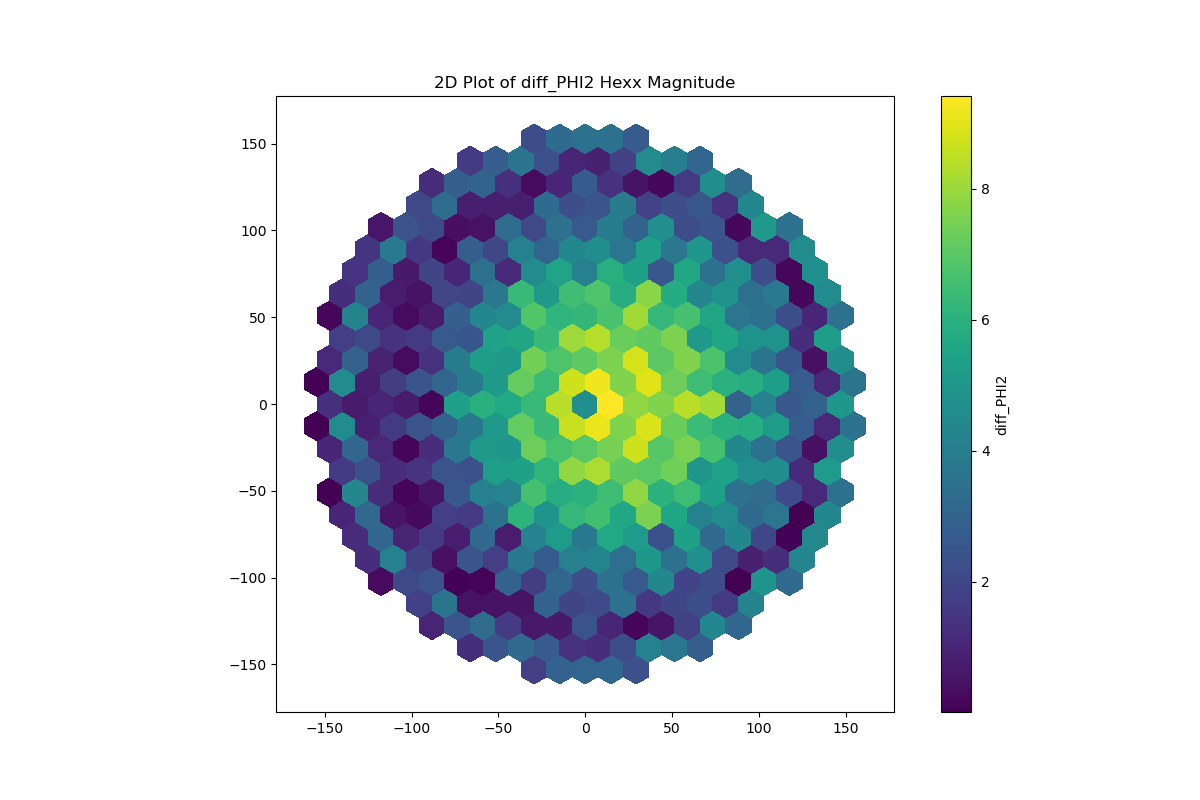
\includegraphics[width=\linewidth]{figures/OBJECTIVES1_TEST05_2DTriMG_VVER400_VandV_level2_FORWARD_diff_PHI_magnitude_G2.png}
        \end{subfigure}
        \caption{Difference of forward flux between FEMFFUSION and the tool}
        \label{fig:2DVVER_fw_results_diff_phi}
\end{figure}

The results show a good agreement between the tool and FEMFFUSION, with a maximum error of 8\% in the forward flux. Overall, the tool is in good agreement with FEMFFUSION.

\section{Conclusion}

A numerical tool has been developed for neutron noise application. The tool is based on the 3-dimensional, multigroup neutron diffusion equation in the frequency domain. The tool can solve rectangular and hexagonal geometries. The tool is designed to solve forward, adjoint, and neutron noise equations with two types of neutron noise sources. It uses sparse matrices to solve systems of linear equations obtained from PETSc. Several cases have been simulated to verify the numerical results against analytical solutions, as well as other tools, such as FEMFFUSION. The results demonstrate that the developed tool aligns with those from analytical solutions and other numerical tools. 
